\chapter{Matériel et Méthode}
La biomasse de zooplancton et micronecton, l'assemblage des communautés phytoplanctoniques, l'environnement physique des organismes ne sont pas directement mesurables, ce sont des construits (\textit{constructs}), c'est à dire des abstractions qui décrivent le phénomène théorique d'intérêt \cite{edwards2000nature}. Pour étudier ces phénomènes, nous avons besoin de trouver des variables mesurables pouvant les décrire, c'est l'opérationnalisation du construit. Les choix des variables utilisées sont justifiées par la connaissances théorique des phénomènes étudiés, appuyés par la littérature. Les variables mesurables sont alors dites variables \textit{proxy} pour les construits associés. \cite{shmueli2010explain}.
 
 
 Les variables proxy sélectionnées sont les suivantes : (1) le Nautical Area Scattering Coefficient(NASC) approxime la biomasse du zooplancton et micronecton sur l'ensemble de la profondeur considérée; (2) les concentrations pigmentaires ($P_1, \ldots, P_9$) approximent l'assemblage des communautés phytoplanctoniques leur abondance totale; (3) le Finite-Time Lyapunov Exponent (FTLE) approxime l'hydrodynamisme et (4) la température et la salinité rendent compte des conditions physico-chimiques du milieu.
 
 Toutes les données utilisées pour cette étude sont des données secondaires, c'est-à-dire que le plan d'échantillonnage n'a pas été construit spécifiquement pour répondre à cette problématique.
 
 \section{Zone d'étude et plan d'échantillonnage}
 
 L'étude a été réalisée sur les années 2018, 2021, 2022 et 2023, en saison estivale (janvier-mars) afin de limiter la variabilité saisonnière, et de jour (calculé selon l'angle solaire), afin de limiter l'effet de la migration verticale journalière (DVM) \footnote{Déplacement synchronisé dans la colonne d'eau au rythme du cycle jour/nuit : les organismes résident en profondeur durant le jour et remontent vers la surface la nuit, principalement pour se nourrir tout en réduisant le risque de prédation visuelle en eaux éclairées. Ce phénomène est considéré comme le plus grand mouvement synchronisé de biomasse à l'échelle de la planète. \cite{Bandara2021}}. La fenêtre d'étude a été fixée à [45,90]°E de longitude et [30, 60]°S de latitude afin de cibler précisémment le secteur indien de l'Océan Austral.
 
 \section{Données d'acoustique active (OBSAUSTRAL) et construction du Nautical Area Scattering Coefficient (NASC)}
 
 \subsection{Données d'acoustique active}
 Les données d'acoustiques actives ont été collectées par transects \footnote{Le bateau se déplace et collecte en même temps des données, par opposition aux données "stations" collectées lorsque le bateau est en arrêt. Cela a un coût en terme de résolution des spectrogramme et d'interprétabilité mais permet d'obtenir une plus grande couverture spatiale.} lors des campagnes océanographiques OBSAUSTRAL/THEMISTO 2018, 2021, 2022, 2023 en saison estivale. Ils sont détaillés sur la figure \ref{fig:transectsparannee2} \cite{flotteoceanographique_campagnes}.  
 \begin{figure}[H]
 	\centering
 	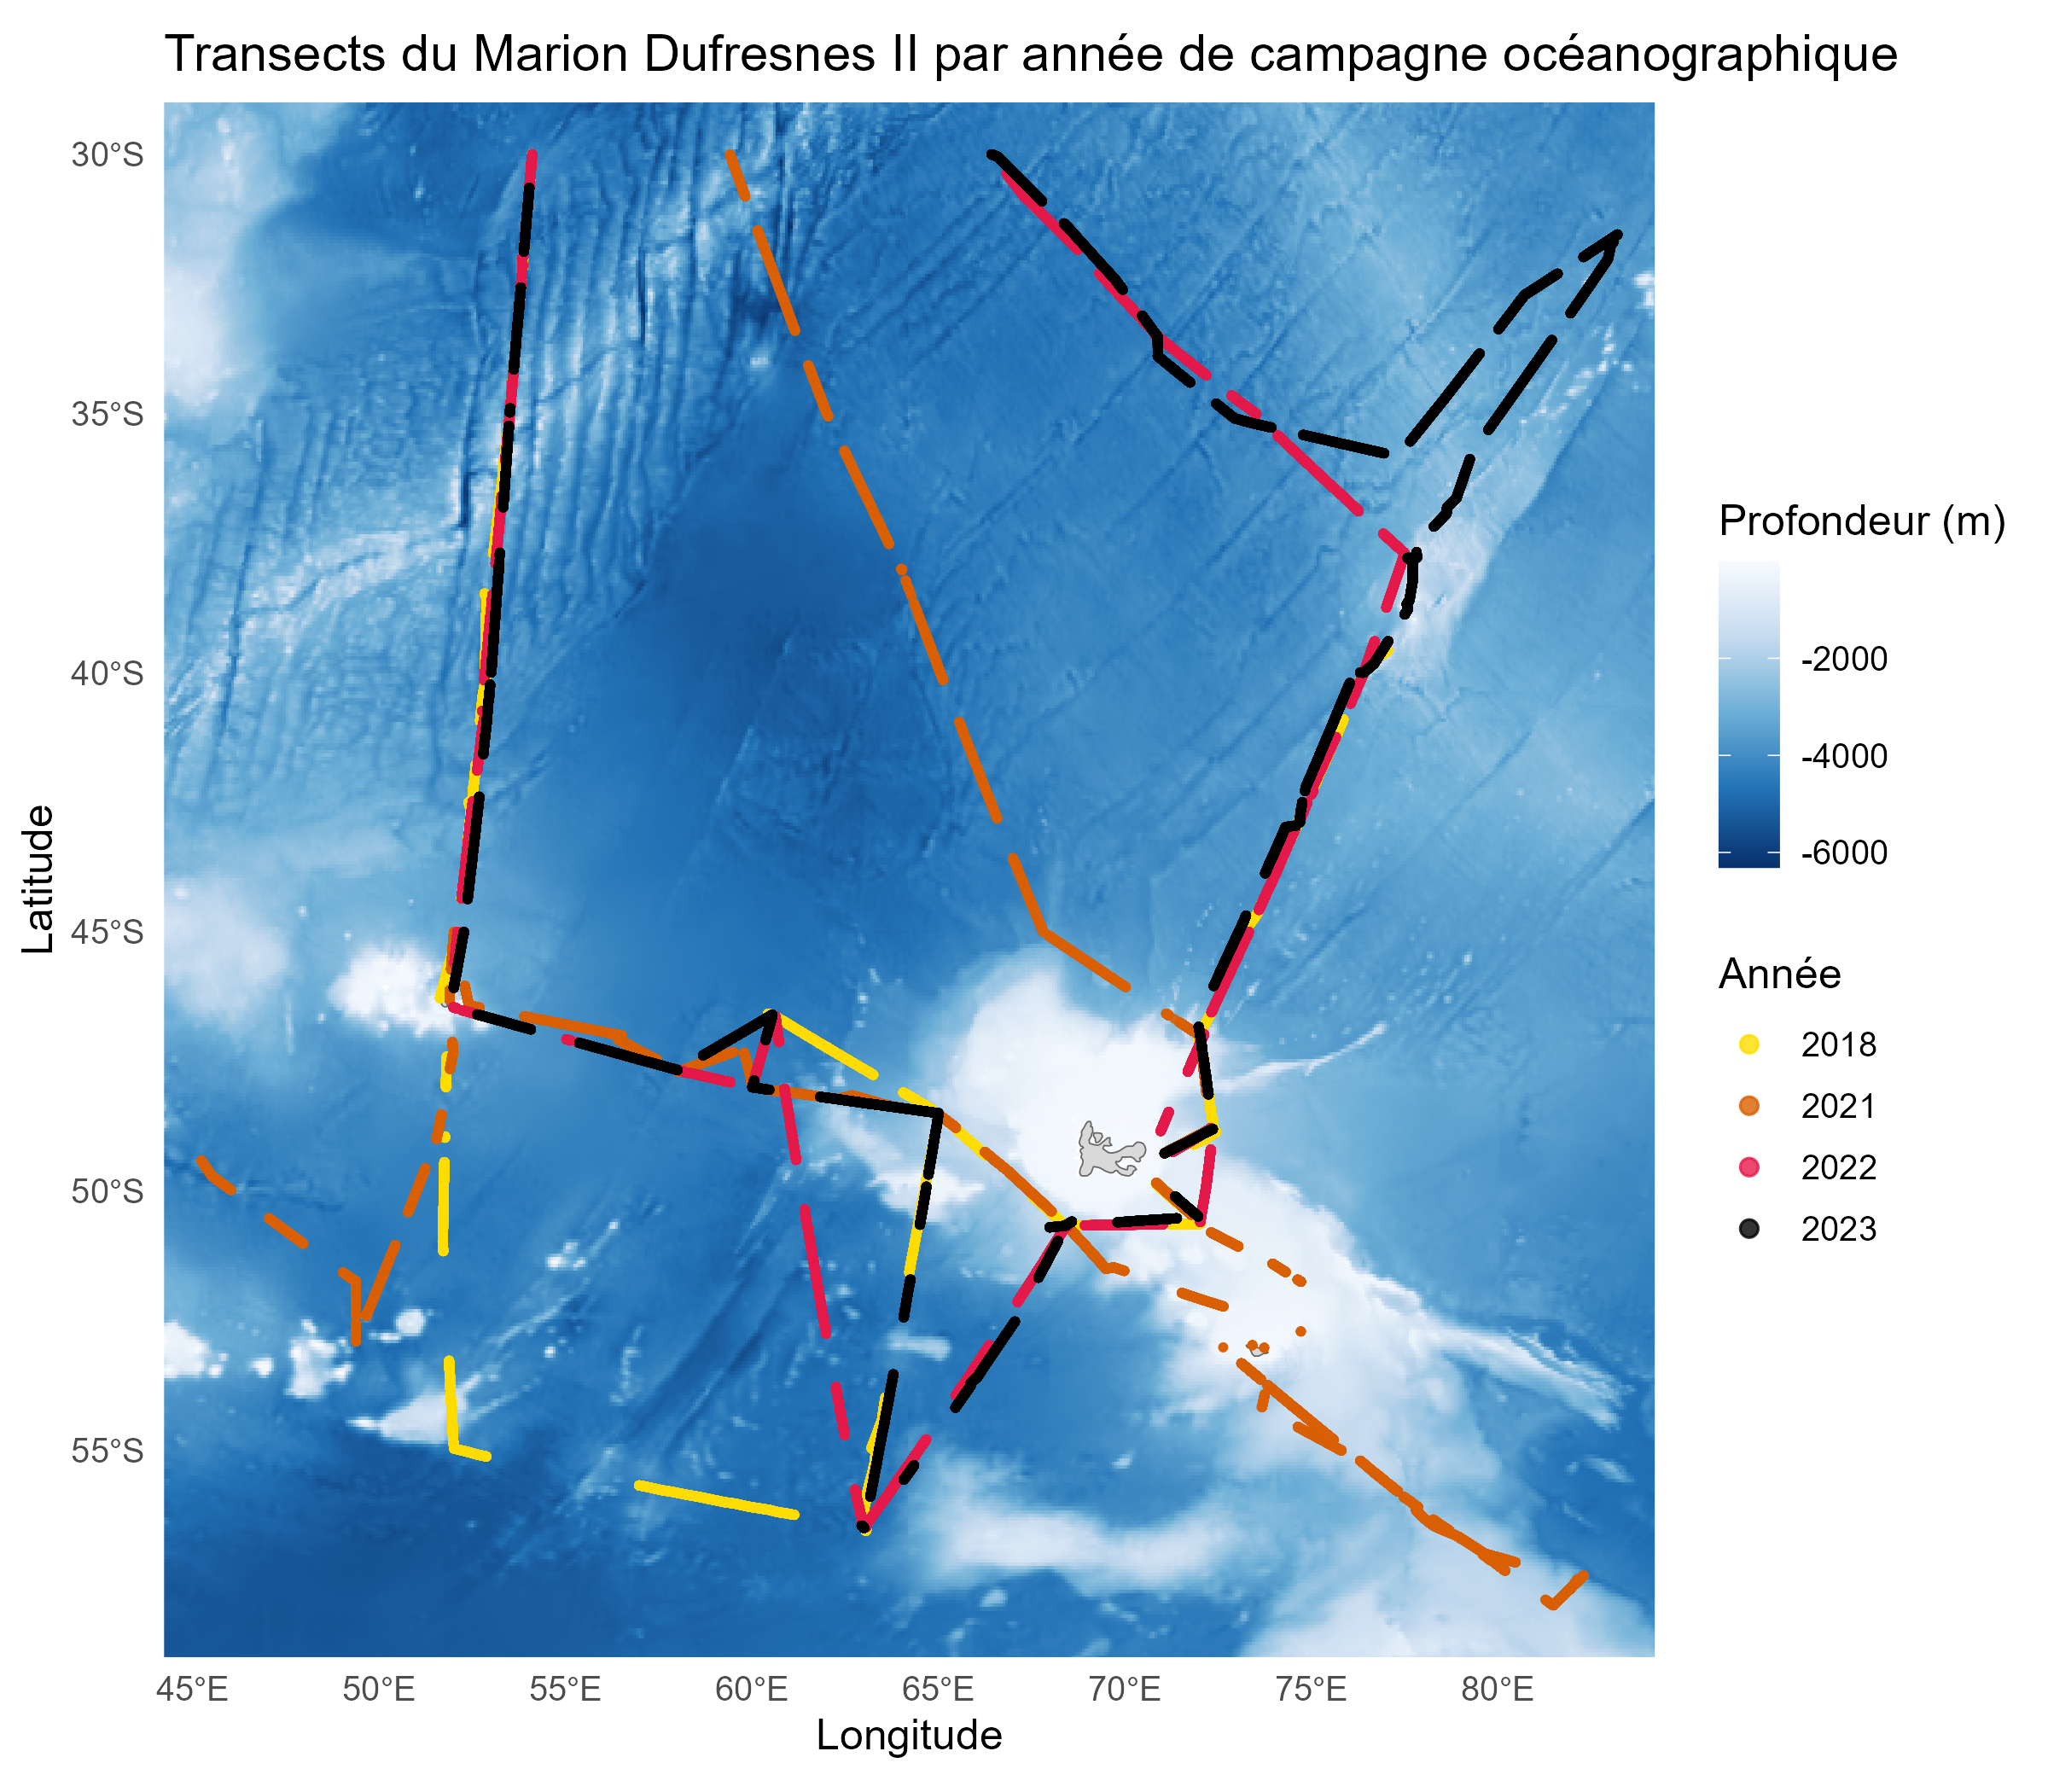
\includegraphics[width=0.6\textwidth]{../images/02_materiel_et_methode/active_acoustic_et_NASC/transects_par_annee_2}
 	\caption{Carte des transects effectués par le Marion Dufresnes II lors des campagnes océanographiques OBSAUSTRAL/THEMISTO 2018, 2021, 2022 et 2023.}
 	\label{fig:transectsparannee2}
 \end{figure}
 
 \vspace{1cm}
 
 Deux fréquences d'émissions ont été sélectionnées: 38 kHz, afin de comparer nos résultats avec la littérature \footnote{La méthode d'acoustique active ayant été développée par les pêcheries, la fréquence d'échosondeur de référence est 38kHz (fréquence à laquelle les poissons sont facilement détectables).} et 120 kHz, fréquence à laquelle les zooplanctons d’intérêts, Euphausiacés (krill) et Copépodes, sont les plus détectables (voir Annexe \ref{annexe:rep_freq}, figure \ref{fig:freqresponse}). Les échogrammes (figures \ref{fig:echogramme38khz2023-01-28} et \ref{fig:echogramme120khz2023-01-28}) donnent un aperçu de la nature des données collectées et de la manière dont l'information contenue par le signal reçu (résolution, organismes visibles) est déterminée par la fréquence de l'onde émise. Une forte intensité de l’écho reçu traduis la présence d'une importante biomasse d'organisme à ce temps, localisation géographique et profondeur.
 
 \begin{figure}[H]
 	\centering
 	\begin{subfigure}[t]{0.7\textwidth}
 		\centering
 		\includegraphics[width=\textwidth]{../images/02\_materiel\_et\_methode/active\_acoustic\_et\_NASC/echogramme\_38kHz\_2023-01-28.png}
 		\caption{Fréquence d'émission de 38 kHz}
 		\label{fig:echogramme38khz2023-01-28}
 	\end{subfigure}
 	\vfill
 	\begin{subfigure}[t]{0.7\textwidth}
 		\centering
 		\includegraphics[width=\textwidth]{../images/02\_materiel\_et\_methode/active\_acoustic\_et\_NASC/echogramme\_120kHz\_2023-01-28.png}
 		\caption{Fréquence d'émission de 120 kHz}
 		\label{fig:echogramme120khz2023-01-28}
 	\end{subfigure}
 	\caption{Exemple d'échogramme obtenu le 2023-01-28 entre 18h et 00h aux fréquences (a) 38 kHz et (b) 120 kHz}
 	\label{fig:echogramme2023-01-28}
 \end{figure}
 
 \subsection{Construction du Nautical Area Scattering Coefficient (NASC)}
 
 L'\textbf{Intensité de l'echo (Echo Level EL) }correspond au signal reçu par le transducteur lorsqu'une onde est émise dans la colonne d'eau puis réfléchis par un objet.
 \begin{equation}
 	EL = SL - 2TL + DI + TS
 \end{equation}	
 où 
 \begin{itemize}
 	\item SL (Source Level): intensité du son émise (dB) $SL = 10 \times \log_{10}(I/I_{ref}) $ et $I_{ref} = \rho_{ref}^{2} = 1 \mu \text{Pa}$ ($\rho_{ref}$ la pression de référence)
 	\item TL (Transmission Loss): perte de transmission  \footnote{Le premier terme correspond à l'attenuation due à la dispersion de l'onde et le second terme correspondant à l'éttenuation de la propagation du milieu ($\alpha$ le coefficient d'absorption en $dB.m^{-1}$)} $TL = 20 \log_{10} (R) + \alpha R$
 	\item DI (Directivity Index): indice de directivité du transducteur (dB)
 	\item TS (Target Strength): réfléctivité de la cible 
 \end{itemize}
 
 \vspace{0.5cm}
 
 La \textbf{section efficace de rétrodiffusion} \(\sigma_{bs} = 10^{\frac{TS}{10}}\)  (\(\mathrm{m^2}\)) caractérise la capacité de la cible à rétrodiffuser l'énergie acoustique. 
 %et est déterminée par référence à la section efficace de rétrodiffusion théorique de la sphère de calibration utilisée lors de la calibration du sondeur. 
 
 \vspace{0.5cm}
 
 Le \textbf{volume backscattering coefficient} $s_v$ (en $m^{2}.m^{-3}$ ou $m^{-1}$) est la somme  toutes les surfaces réfléctives $\sigma_{bs}$ de toutes les cibles acoustiques dans le volume d'échantillonage $V_0$, normalisées à 1$m^{3}$.  
 \begin{equation}
 	s_v = \sum \sigma_{bs}/V
 \end{equation}
 Il mesure la densité acoustique des organismes présents dans un volume d'eau. Un niveau de $s_v$ élevé correspond à une quantité plus importante de rétrodiffusion acoustique dans le volume échantillonné. Ce qui est interprété comme un nombre important d'organismes présents dans la colonne d'eau ou un organisme de taille importante ou encore un organisme ayant des propriétés fortement retrodiffusantes \footnote{Beaucoup de poissons pélagiques ont des vessies natatoires remplie de gaz ou de graisse, ce sont des organes leur permettant d'ajuster leur flottabilité. Cette vessie natatoire est connue pour particulièrement retrodiffuser à 38kHz et donc augmenter le signal}. Par convention, on exprime souvent cette grandeur en échelle logarithmique sous le nom de Volume Backscattering Strength, noté $S_v \text{ (dB re 1 m}^{-1})$ tel que $s_v = 10^{\frac {S_v} {10}}$.
 
 \vspace{0.5cm}
 
 Le \textbf{Nautical Area Scattering Coefficient (NASC)}, noté $s_A$, correspond au coefficient de rétrodiffusion acoustique par unité de surface nautique (en $m^{2}.nmi^{-2}$). Il résume la rétrodiffusion acoustique sur une couche d'eau donnée en intégrant entre deux profondeurs le volume backscattering coefficient $s_v$ multiplié par un certain facteur (convention) :
 \begin{equation}
 	s_A = 4 \pi (1852)^{2} \int_{z_{1}}^{z_{2}} s_v(z) dz
 \end{equation}
 
 Dans le cadre de cette étude, la profondeur d'intégration $z_1$ a été fixé à 25 m pour limiter le bruit d’échantillonnage de surface \footnote{effet de "bullage" du bateau bruitant les données à des faibles profondeurs}. Le choix de $z_2$ dépend de la fréquence de l'échosondeur : pour des fréquences de 38 kHz et 120 kHz, la colonne d'eau est échantillonné respectivement jusqu'à une profondeur moyenne de 700 m et 300 m. En effet, à partir de ces profondeurs, beaucoup de données $s_v$  sont manquantes (voir Annexe \ref{annexe:missing_values}, figure \ref{fig:diagnabydepthperesu}). Les profils avec plus de 50\% de valeurs manquantes ont été exclus du jeu de données. Les valeurs manquantes résiduelles ont été comblées : (1) par interpolation linéaire lorsque situées entre deux valeurs connues et (2) par prolongation de la valeur la plus proche, lorsque situées aux extrémités. 
 
 \vspace{0.5cm}
 
 Ainsi, pour chaque profil de $S_v$, on calcule le NASC et obtenons un scalaire, qui résume le volume de rétrodiffusion acoustique sur l'ensemble de la couche d'eau considérée ([25-700]m pour 38kHz et [25-300]m pour 120kHz). La figure \ref{fig:diagnasctimeperesu120khz2023}) présente le NASC en fonction du temps pour le transect 2023 OBSAUSRAL.
 
 \begin{figure}[H]
 	\centering
 	\includegraphics[width=0.7\textwidth]{images/03_methodology/nasc_2023-01-28_smooth_bis.png}
 	\caption{NASC en fonction du temps le 2023-01-28, données d'acoustique active (transect) issues de la campagne océanographique OBSAUSTRAL 2023 \cite{flotteoceanographique_campagnes}.}
 	\label{fig:diagnasctimeperesu120khz2023}
 \end{figure}
 
 
 
 
 
 
 
 
 
 \section{Concentrations de pigments photosynthétiques (PIGMeANN)}
 L'analyse de la couleur des océans à partir d'images satellite permet de d'étudier le phytoplancton sur une échelle spatiale et temporelle large. Des méthodes de machine learning et, plus récemment de deep learning, ont permis la caractérisation de "Phytoplankton Functional Types" et de "Phytoplakton Size Classes"  depuis des images satellites \cite{Alvain2005}, \cite{Li2023DLPPCE}, \cite{Waga2026CSD}.  Les spectres de reflectance des océans dépendent des pigments photosynthétiques qu'ils contiennent. L'idée est d'identifier une empreinte spectrale et de l'associer (par deep learning) avec des mesures \textit{in-situ} de High Performance Liquid Chromatography \footnote{L’échantillon est injecté dans une colonne traversée par un solvant sous haute pression, où ses différents composés sont séparés puis détectés individuellement. Permet de séparer et quantifier les pigments afin d’identifier les différents groupes présents.} et de cytométrie en flux\footnote{Les cellules sont entraînées individuellement devant un laser qui mesure leur diffusion (taille/forme des cellules) et leur fluorescence. On peut ensuite identifier les taxons.} qui caractérisent plus précisemment la présence et structure des communauté phytoplanctoniques. 
 \begin{table}[H]
 	\centering
 	\renewcommand{\arraystretch}{1.3}
 	\begin{tabular}{
 			>{\raggedright\arraybackslash}p{3.4cm}
 			>{\raggedright\arraybackslash}p{2.0cm}
 			>{\raggedright\arraybackslash}p{4.8cm}
 			>{\raggedright\arraybackslash}p{2.6cm}
 		}
 		\hline
 		\textbf{Pigment} & \textbf{Abréviation} & \textbf{Groupe phytoplanctonique associé (PFD)} & \textbf{Classe de taille (PSC)} \\
 		\hline
 		Divinyl chlorophylle $a$ & dvChla & Procaryotes picoplanctoniques (\textit{Prochlorococcus}) & Picophytoplancton \\
 		Chlorophylle $a$ & Chla & Marqueur de biomasse totale (tous groupes) & -- \\
 		Chlorophylle $b$ & Chlb & Chlorophycées / Prasinophycées & Picophytoplancton \\
 		Zéaxanthine & Zea & Cyanobactéries (\textit{Synechococcus}) & Picophytoplancton \\
 		Fucoxanthine & Fuco & Diatomées (dominantes) & Microphytoplancton \\
 		19'-hexanoyloxyfucoxanthine & Hex & Prymnésiophycées (haptophytes) & Nanophytoplancton \\
 		19'-butanoyloxyfucoxanthine & But & Prymnésiophycées / pélagophytes & Nanophytoplancton \\
 		Alloxanthine & Allo & Cryptophycées & Nanophytoplancton \\
 		Péridinine & Per & Dinoflagellés (péridiniens) & Microphytoplancton \\
 		\hline
 	\end{tabular}
 	\renewcommand{\arraystretch}{1}
 	\caption{Pigments photosynthétiques analysés et groupes phytoplanctoniques hypothétiquement associés (PFD et PSC) dans le secteur de Kerguelen en été austral, d'après \cite{Lasbleiz2014}, \cite{sari2025influence}}
 	\label{tab:pigments}
 \end{table}
 
 La méthode de deep-learning PIGMeANN a récemment été développée \cite{sari2026regional} : elle permet d'approximer les concentrations de surface de neuf pigments photosynthétiques (tableau \ref{tab:pigments}) sur l'ensemble de la couverture spatiale de l'image satellite donnée en entrée. La figure  \ref{fig:mapchla2023-01-26} illustre la prédiction par PIGMeANN de la Chorophylle-a le 2023-01-26 sur le secteur étudié.
 
 \begin{figure}[H]
 	\centering
 	\includegraphics[width=0.7\textwidth]{images/02_materiel/map_chla_2023-01-26}
 	\caption{Carte de prédiction de la concentration de Chlorophylle-a le 2023-01-26 sur le secteur indient du SO, prédictions issue de l'alorithme PIGMeANN développé par Sari el Dine \cite{sari2026regional}. La présence de nuages gène grandement la prédiction sur la zone totale.}
 	\label{fig:mapchla2023-01-26}
 \end{figure}
 
 A partir de la connaissance des différentes communautés phytoplanctoniques présente dans la région d'étude, on peut hypothétiquement associer certains pigments à des groupes phytoplanctoniques (PFD) ou Phytoplankton Size Classes (PSC) (voir tableau \ref{tab:pigments})\cite{sari2025influence}, \cite{heidemann2024drivers} \cite{Georges2014}. Ces associations permettent alors, à partir des assemblage de concentration de pigments photosynthétiques prédits par PIGMeANN, de caractériser les structures des communautés phytoplanctoniques en identifiant les PFD et PSC dominantes. 
 
 La chlorophylle-a, utilisée comme proxy de la biomasse phytoplanctonique totale, est exclue de cette identification car peu discriminante : présente à forte concentration chez la quasi-totalité des organismes, elle n'apporte pas d'information sur la composition de la communauté. Pour chaque pigment restant, on calcule donc sa contribution relative (ratio par rapport à la somme des pigments) plutôt que sa concentration absolue :
 
 \begin{equation}
 	R_i = \frac{[\text{Pigment}_i]}{\displaystyle\sum_{j \neq \text{Chla}} [\text{Pigment}_j]}
 	\label{eq:ratio_pigment}
 \end{equation}
 
 \section{Données hydrologiques de température et salinité (CMEMS)}
 Les données de températures et salinité sont issues de la plateforme Copernicus \footnote{Programme d’observation de la Terre de l’Union européenne, qui fournit notamment des données et services permettant de surveiller et comprendre l’état de l’environnement, dont l’océan \cite{copernicus2026services}}. Ce sont des données issues des observations temps-réelles CMEMS \footnote{Copernicus Marine Environment Monitoring Service, service marin de Copernicus} et réanalysées par le modèle NEMO \footnote{Nucleus for European Modelling of the Ocean, modèle numérique de l’océan qui simule l’évolution de paramètres comme la température, la salinité, les courants et le niveau de la mer}, et ERA5 \footnote{Modèle atmosphérique de l'ECMWF (European Centre for Medium-Range Weather Forecasts) qui fournit les conditions atmosphériques nécessaires pour forcer le modèle océanique NEMO à sa surface}. Elles ont une résolution spatiale de 0.083° et une résolution temporelle journalière.
 Sont téléchargés tous les profils de température et de salinité de la zone d'étude (entre 45-90°E de longitude et 30 et 60°S de latitude), sur l'ensemble de la période étudiée (2018, 2021, 2022, 2023, entre janvier et mars). 
 
 \section{Données hydrodynamiques : Finite Time Lyapunov Exponent}
 Le Finite Time Lyapunov Exponent est un indicateur qui, à partir de champs de courants estimés par modélisation, permet de caractériser la séparation ou la convergence de trajectoires de particules d’eau sur une durée finie. On peut ainsi identifier les structures dynamiques susceptibles de contrôler le transport et la dispersion dans l’océan \cite{shadden2005definition}, \cite{dovidio2004mixing}. Son calcul est détaillé en Annexe \ref{annexe:compute_ftle}.
 
 \vspace{0.5em}
 
 \begin{figure}[H]
 	\centering
 	\includegraphics[width=0.5\textwidth]{images/02_materiel/map_ftle_2023-01-26}
 	\caption{Advection Lagrangienne FTLE backward (90j) du 2023-01-26. Les valeurs élevées de FTLE délimitent des crêtes correspondant  à des frontières de transport de l'écoulement (de fronts ou de tourbillons) le long desquelles convergent les masses d'eau (structures cohérentes lagrangiennes attractives)}
 	\label{fig:mapftle2023-01-26}
 \end{figure}
 
 Dans notre étude, la durée d'advection est de trente jours en backward, c'est-à-dire que les trajectoires sont intégrées vers l'arrière dans le temps (de $t$ à $t - T$). La résolution temporelle est journalière et la résolution spatiale est de 0.05°.On obtient des cartes de FTLE $\in \mathbb{R}^{time \times lon \times lat}$ pour la période (2018, 2021, 2022, 2023 entre janvier et mars) et région étudiée ([45, 90]°E, [30, 60]°S). 
 
 La figure \ref{fig:mapftle2023-01-26} présente une carte de FTLE issue de la journé 2023-01-26. Une valeur élevée du FTLE indique une forte séparation des trajectoires voisines sur la période considérée. Les structures organisées apparaissant comme des crêtes de FTLE peuvent ainsi être utilisées pour identifier des structures physiques réelles dans l'écoulement océanique, appelées Structures Cohérentes Lagrangiennes \cite{shadden2005definition}.